\documentclass[11pt,a4paper]{article}
\usepackage[utf8]{inputenc}
\usepackage[T1]{fontenc}
\usepackage{tgpagella}
\usepackage[spanish]{babel}
\usepackage{geometry}
\usepackage{booktabs}
\usepackage{xcolor}
\usepackage{titlesec}
\usepackage{fancyhdr}
\usepackage[parfill]{parskip}
\usepackage[expansion=false]{microtype}
\usepackage{hyperref}
\usepackage{setspace}
\usepackage{graphicx}
\usepackage{needspace}

\widowpenalty=10000
\clubpenalty=10000
\displaywidowpenalty=10000

\geometry{top=3.0cm,bottom=3.0cm,left=3.5cm,right=3.5cm}
\setlength{\parskip}{0.65em}
\setlength{\parindent}{0em}

\definecolor{azulai}{RGB}{30,80,140}
\definecolor{doradoai}{RGB}{140,90,0}
\definecolor{grisai}{RGB}{70,70,70}

\titleformat{\section}{\Large\bfseries\color{azulai}}{}{0em}{}[{\color{azulai}\titlerule[0.5pt]}]
\titlespacing*{\section}{0pt}{1.4em}{0.5em}

\titleformat{\subsection}{\large\bfseries\color{doradoai}}{}{0em}{}
\titlespacing*{\subsection}{0pt}{1.0em}{0.35em}

\titleformat{\subsubsection}{\normalsize\bfseries\color{grisai}}{}{0em}{}
\titlespacing*{\subsubsection}{0pt}{0.7em}{0.25em}

\pagestyle{fancy}\fancyhf{}
\rhead{\textcolor{grisai}{\small Raquel Pain — Arquitectura Interna}}
\lhead{\textcolor{grisai}{\small Plutón · Casa 8 · Casa 12 · Quirón · Lilith}}
\cfoot{\textcolor{grisai}{\small\thepage}}
\renewcommand{\headrulewidth}{0.3pt}

\hypersetup{colorlinks=true,linkcolor=azulai,urlcolor=azulai}
\setstretch{1.25}
\tolerance=1500
\emergencystretch=4em

\begin{document}

\begin{titlepage}
  \centering
  \vspace*{1.5cm}
  {\Huge\bfseries\color{azulai} Plutón · Casa 8 · Casa 12}\\[0.35cm]
  {\Huge\bfseries\color{azulai} Quirón · Lilith}\\[0.5cm]
  {\large\color{grisai} Arquitectura Interna}\\[0.3cm]
  {\small\itshape\color{grisai} Sombra, herida, intimidad y profundidad psíquica}\\[2cm]
  {\huge\color{doradoai} Raquel Pain}\\[1.5cm]
  {\Large 07/05/1985 \quad 18:20}\\[0.3cm]
  {\Large Pamplona, España}\\[0.3cm]
  {\normalsize Lat: 42.8157° \quad Lon: -1.6522° \quad UTC+02:00}\\[0.3cm]
  {\normalsize Ascendente: Libra 14°36' \quad
    MC: Cáncer 17°21'}\\[2cm]

  \begin{tabular}{ll}
    \textbf{Plutón:}  & Escorpio — Casa 1 2°58' (retrógrado) \\
    \textbf{Quirón:}  & Géminis — Casa 8 7°04' \\
    \textbf{Lilith:}  & Aries — Casa 7 27°13' \\
    \textbf{Casa 8:}  & Tauro \\
    \textbf{Casa 12:} & Virgo \\
  \end{tabular}\\[2cm]

  \vfill
  {\small Generado el 20/05/2026}
\end{titlepage}

\tableofcontents
\newpage

\section{Datos de referencia}

\begin{center}
\begin{tabular}{llll}
  \toprule
  \textbf{Punto} & \textbf{Signo} & \textbf{Casa} & \textbf{Posición} \\
  \midrule
  Plutón (retrógrado) & Escorpio & 1 & 2°58' \\
  Quirón & Géminis & 8 & 7°04' \\
  Lilith          & Aries & 7 & 27°13' \\
  Casa 8          & Tauro             & ---                  & --- \\
  Casa 12         & Virgo            & ---                  & --- \\
  Ascendente      & Libra         & ---                  & 14°36' \\
  Medio Cielo     & Cáncer          & ---                  & 17°21' \\
  \bottomrule
\end{tabular}
\end{center}

\vspace{0.5cm}
\textbf{Aspectos relevantes:}

\begin{center}
\begin{tabular}{lllll}
  \toprule
  \textbf{Punto 1} & \textbf{Asp.} & \textbf{Punto 2} & \textbf{Aspecto} & \textbf{Orbe} \\
  \midrule
  Plutón & sex & Neptuno & Sextil & 0.4° \\
  Quirón & conj & Marte & Conjunción & 0.7° \\
  Quirón & sex & Venus & Sextil & 1.8° \\
  Lilith & tri & Luna & Trígono & 0.7° \\
  \bottomrule
\end{tabular}
\end{center}

\begin{center}
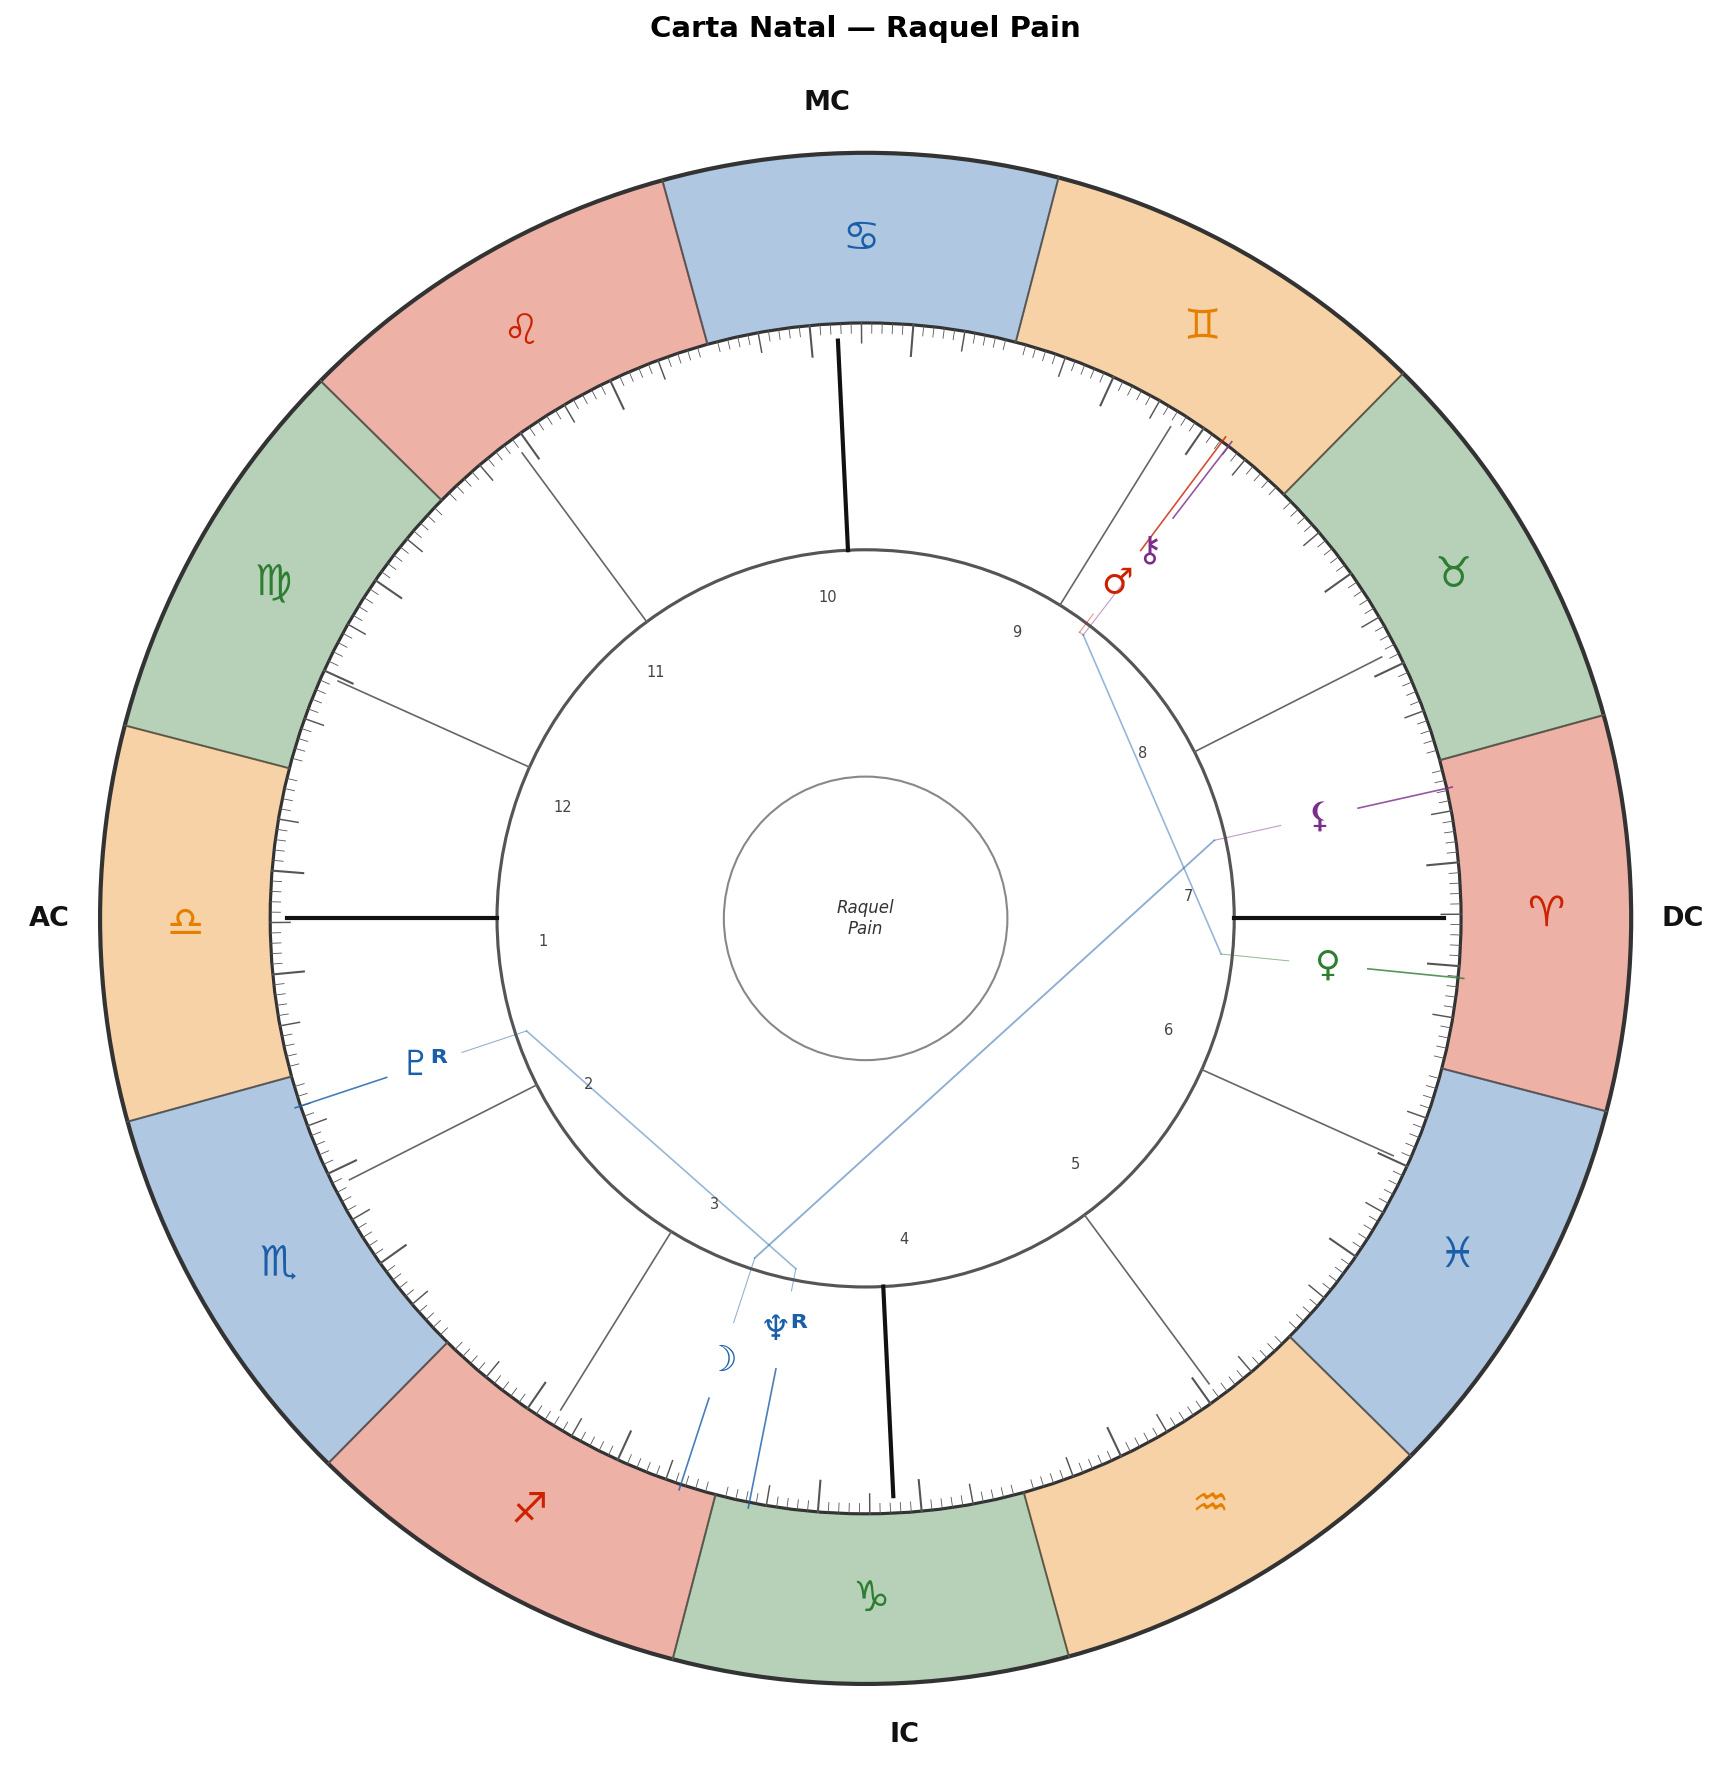
\includegraphics[width=0.72\textwidth]{Raquel_Pain_rueda.png}
\end{center}

\Needspace{3\baselineskip}

\section{Interpretación}

\begin{center}
{\small\itshape
Este documento no busca definirte. Se acerca a zonas donde pueden aparecer intensidad,\\
defensa, herida, vulnerabilidad, deseo, retiro o dificultad para poner en palabras lo que ocurre.
}
\end{center}

\vspace{0.8cm}

\Needspace{10\baselineskip}
\vspace{0.4cm}

\subsection{1. Marco general}

Este documento entra en zonas de la carta que suelen vivirse con más intensidad, más defensa o más dificultad para nombrar. No describe una identidad fija ni una condena personal. Se acerca a lugares donde pueden aparecer miedo, control, vergüenza, deseo, aislamiento, dependencia, heridas antiguas o reacciones difíciles de comprender desde fuera.

Plutón en Escorpio, Casa 1: muestra dónde puedes vivir procesos intensos de transformación, pérdida de control, apego, defensa o profundidad emocional.
Quirón en Géminis, Casa 8: muestra una zona especialmente sensible, donde puede haber herida, inseguridad, vergüenza o necesidad de protección.
Lilith en Aries, Casa 7: muestra una parte de ti menos domesticable, más instintiva, que puede reaccionar con fuerza cuando se siente atrapada, reducida o invadida.

La Casa 8 en Tauro habla de cómo atraviesas la vulnerabilidad, la intimidad, la pérdida, la confianza y los vínculos que remueven profundamente.
La Casa 12 en Virgo habla de cómo vives el retiro, la sensibilidad, el agotamiento emocional, lo inconsciente y aquello que cuesta poner en palabras.

Aspectos principales observados en este bloque: Plutón–Neptuno en sextil (orbe 0.37°), Quirón–Marte en conjunción (orbe 0.74°), Quirón–Venus en sextil (orbe 1.79°), Lilith–Luna en trígono (orbe 0.7°).

\Needspace{10\baselineskip}
\vspace{0.4cm}

\subsection{2. Plutón — Intensidad, control y transformación}

\Needspace{6\baselineskip}
\subsubsection*{Plutón en Escorpio — Casa 1 (retrógrado)}

Plutón en Escorpio intensifica los temas propios de Plutón: deseo, control, pérdida, intimidad, miedo, poder y transformación. Puede haber una vida interna muy profunda, con emociones que rara vez son superficiales o fáciles de atravesar.

La sombra puede aparecer como obsesión, desconfianza, necesidad de controlar, dificultad para soltar o tendencia a vivirlo todo con una intensidad extrema. A veces puedes detectar la herida ajena con mucha claridad, pero proteger ferozmente la tuya.

La transformación pasa por dejar de confundir intensidad con verdad absoluta. Tu poder crece cuando puedes entrar en lo profundo sin quedarte atrapade en la herida.

Plutón en casa 1 suele dar una presencia intensa, incluso cuando no intentas llamar la atención. Muchas veces las personas perciben algo fuerte en ti antes de que hayas dicho demasiado.

Puede haber necesidad de controlar cómo te muestras, dificultad para sentirte vulnerable o sensación de tener que sostenerte con mucha fuerza frente al mundo. A veces atraviesas cambios profundos de identidad que hacen que ciertas versiones de ti ya no puedan mantenerse.

La transformación pasa por dejar de vivir la exposición como amenaza constante. Tu presencia se vuelve más sólida cuando no necesitas protegerla todo el tiempo.

Plutón está retrógrado. La intensidad tiende a dirigirse primero hacia dentro. Puede haber procesos profundos que no se ven claramente desde fuera, pero que por dentro acumulan mucha fuerza. A veces tardas en mostrar lo que está ocurriendo, aunque internamente algo ya esté transformándose.

Plutón–Neptuno en sextil (orbe 0.37°).
Plutón en aspecto con Neptuno intensifica la sensibilidad, la percepción profunda y la relación con lo invisible o difícil de explicar. Puede haber mucha permeabilidad emocional, intuición o dificultad para distinguir entre deseo, miedo y fantasía.

A veces necesitas poner límites claros a lo que absorbes o idealizas.

El sextil abre una posibilidad de aprendizaje consciente. Puede no activarse solo, pero cuando le prestas atención permite trabajar esta combinación de una forma más manejable.

Este aspecto es muy cerrado, por lo que suele sentirse con bastante fuerza. No aparece como algo lejano o secundario, sino como una dinámica que puede activarse con claridad en momentos importantes.

\Needspace{10\baselineskip}
\vspace{0.4cm}

\subsection{3. Quirón — Herida, sensibilidad y protección}

\Needspace{6\baselineskip}
\subsubsection*{Quirón en Géminis — Casa 8}

Quirón en Géminis suele mostrar sensibilidad en torno a la palabra, la comunicación y la sensación de que te comprendan. Puede haber miedo a expresarte mal, decir algo incorrecto o sentir que tu forma de pensar no encaja del todo.

A veces observas demasiado cómo hablas, explicas o respondes. También puede aparecer dificultad para confiar en tu propia percepción, especialmente si creciste sintiendo que lo que pensabas era minimizado o cuestionado.

El aprendizaje pasa por permitirte comunicar desde un lugar más vivo y menos defensivo. Tu voz gana fuerza cuando deja de intentar protegerse constantemente.

Quirón en casa 8 suele mostrar heridas profundas ligadas a la vulnerabilidad, la intimidad y la confianza emocional. Puede costarte abrir ciertas partes de ti porque la exposición emocional se siente especialmente delicada.

A veces deseas mucha cercanía pero al mismo tiempo aparece miedo intenso a depender, perder control o que te dañen. También puede existir tendencia a proteger lo más sensible de forma muy silenciosa.

El aprendizaje pasa por descubrir que abrirte emocionalmente no implica necesariamente quedar indefense.

Quirón–Marte en conjunción (orbe 0.74°).
Quirón en aspecto con Marte toca la acción, la rabia, la defensa y la capacidad de afirmarte. Puede haber miedo al conflicto, dificultad para poner límites o sensación de que tu fuerza no es segura.

A veces contienes demasiado hasta que la energía sale de golpe.

La conjunción intensifica mucho esta combinación. Ambas partes tienden a mezclarse, por lo que puede costar separarlas o tomar distancia de lo que activan juntas.

Este aspecto es muy cerrado, por lo que suele sentirse con bastante fuerza. No aparece como algo lejano o secundario, sino como una dinámica que puede activarse con claridad en momentos importantes.

Quirón–Venus en sextil (orbe 1.79°).
Quirón en aspecto con Venus toca heridas vinculadas al amor, el deseo, el merecimiento y la capacidad de recibir. Puede haber miedo al rechazo, dificultad para sentirte elegide o tendencia a adaptarte demasiado para conservar afecto.

A veces cuesta creer que pueden quererte sin tener que ganártelo continuamente.

El sextil abre una posibilidad de aprendizaje consciente. Puede no activarse solo, pero cuando le prestas atención permite trabajar esta combinación de una forma más manejable.

El orbe es relativamente cercano, así que esta combinación puede sentirse de forma bastante reconocible.

\Needspace{10\baselineskip}
\vspace{0.4cm}

\subsection{4. Lilith — Lo no domesticado}

\Needspace{6\baselineskip}
\subsubsection*{Lilith en Aries — Casa 7}

Lilith en Aries muestra una parte de ti muy instintiva, directa y difícil de contener cuando siente amenaza o limitación. Puede haber rechazo profundo a sentir que te controlan, frenan o ser dependiente.

A veces reaccionas antes de pensar demasiado porque algo dentro necesita proteger su autonomía rápidamente. También puede aparecer rabia acumulada cuando llevas mucho tiempo cediendo, adaptándote o conteniéndote.

El aprendizaje pasa por relacionarte con tu fuerza sin convertir cada límite o desacuerdo en una lucha constante.

Lilith en casa 7 muestra intensidad en los vínculos y sensibilidad muy fuerte respecto a las dinámicas de dependencia, control o pérdida de libertad. Puede haber una parte de ti que desea mucha cercanía y al mismo tiempo teme profundamente quedar atrapade dentro de la relación.

A veces necesitas tomar distancia cuando el vínculo se vuelve demasiado invasivo o emocionalmente exigente. También puede aparecer atracción hacia relaciones intensas donde se activan dinámicas de poder difíciles de sostener.

El aprendizaje pasa por permitir vínculo sin sentir que necesitas desaparecer o defenderte constantemente.

Lilith–Luna en trígono (orbe 0.7°).
Lilith en aspecto con la Luna intensifica la vida emocional y la necesidad de protección interna. Puede haber sensibilidad extrema al abandono, la invasión emocional o la dependencia.

A veces deseas cercanía y al mismo tiempo reaccionas fuerte cuando algo se acerca demasiado.

El trígono facilita que esta combinación fluya con más naturalidad. No elimina la profundidad del aspecto, pero puede hacer que encuentres recursos internos con mayor facilidad.

Este aspecto es muy cerrado, por lo que suele sentirse con bastante fuerza. No aparece como algo lejano o secundario, sino como una dinámica que puede activarse con claridad en momentos importantes.

\Needspace{10\baselineskip}
\vspace{0.4cm}

\subsection{5. Casa 8 — Intimidad, pérdida y vulnerabilidad}

\Needspace{6\baselineskip}
\subsubsection*{Casa 8 en Tauro}

La casa 8 en Tauro suele vivir los procesos emocionales profundos de manera lenta pero muy intensa. Puede haber mucho apego a lo que da seguridad, especialmente en vínculos importantes.

A veces cuesta soltar relaciones, dinámicas o formas de sostén emocional incluso cuando ya generan sufrimiento. También puede aparecer miedo fuerte a la pérdida, al cambio o a la sensación de inestabilidad.

El aprendizaje pasa por descubrir que abrirte al cambio no implica perder completamente el suelo bajo los pies.

En tu carta, la Casa 8 contiene los siguientes planetas o puntos: Sol, Marte, Quirón.

Sol en Casa 8.
El Sol en casa 8 suele vivir la identidad de forma intensa y transformadora. Las experiencias importantes rara vez pasan por tu vida sin dejar huella profunda.

Puede haber necesidad de comprender lo que ocurre por debajo de la superficie y dificultad para sostener relaciones completamente superficiales. También puede aparecer miedo a perder control emocional o sensación de quedar demasiado expueste cuando algo te importa de verdad.

El aprendizaje pasa por descubrir que mostrar vulnerabilidad no disminuye tu fuerza.

Marte en Casa 8.
Marte en casa 8 suele contener mucha intensidad emocional y energética. Puede haber reacciones muy fuertes cuando sientes amenaza, pérdida de control o vulnerabilidad.

A veces acumulas tensión durante mucho tiempo hasta que termina saliendo de golpe. También puede aparecer necesidad de controlar emocionalmente ciertas situaciones para no sentirte expueste o indefense.

El aprendizaje pasa por reconocer antes lo que ocurre dentro de ti sin esperar siempre al límite.

Quirón en Casa 8.
Quirón en casa 8 suele mostrar heridas profundas ligadas a la confianza, la intimidad y la exposición emocional. Puede costarte abrir ciertas partes de ti por miedo a que te dañen, rechacen o malinterpreten.

A veces deseas mucha cercanía mientras otra parte de ti se protege constantemente de ella. También puede haber sensibilidad muy fuerte respecto a pérdida, dependencia o traición.

El aprendizaje pasa por permitir vulnerabilidad sin sentir que eso te deja indefense.

\Needspace{10\baselineskip}
\vspace{0.4cm}

\subsection{6. Casa 12 — Retiro, sensibilidad y mundo interno}

\Needspace{6\baselineskip}
\subsubsection*{Casa 12 en Virgo}

La casa 12 en Virgo suele vivir mucho cansancio interno ligado a la autoexigencia, el control y la necesidad de sostenerlo todo correctamente. Puede costarte descansar de verdad porque siempre hay algo pendiente de resolver.

A veces intentas ordenar mentalmente emociones que en realidad necesitan ser escuchadas o atravesadas. También puede aparecer ansiedad silenciosa respecto al cuerpo, el rendimiento o la sensación de no llegar suficientemente bien.

El aprendizaje pasa por permitirte imperfecta sin sentir que todo se derrumba por ello.

En tu carta no hay planetas principales dentro de la Casa 12. Aun así, esta casa sigue hablando de cómo vives el retiro, la sensibilidad, el agotamiento emocional y aquello que cuesta poner en palabras.

\Needspace{10\baselineskip}
\vspace{0.4cm}

\subsection{7. Integración}

En conjunto, este bloque muestra una zona de lectura especialmente profunda de la carta. Plutón en Escorpio, Casa 1, señala dónde la intensidad puede obligarte a atravesar procesos de transformación real. Quirón en Géminis, Casa 8, muestra una sensibilidad que no siempre se deja tocar fácilmente. Lilith en Aries, Casa 7, señala una parte de ti que no acepta ser reducida, controlada o domesticada sin reaccionar.

La Casa 8 en Tauro describe cómo te acercas a la intimidad, la pérdida de control, la confianza y los vínculos que remueven. La Casa 12 en Virgo muestra cómo se viven el cansancio profundo, el retiro, la sensibilidad y aquello que a veces permanece oculto incluso para ti.

Las conjunciones intensifican mucho lo que tocan. Cuando Plutón, Quirón o Lilith están unidos a otro punto de la carta, esa parte de ti puede vivirse con más profundidad, más sensibilidad o más dificultad para tomar distancia.

Los aspectos fluidos muestran recursos internos para atravesar estas zonas con más naturalidad. No eliminan la intensidad, pero pueden facilitar comprensión, integración y mayor honestidad contigo.

La clave de este documento no es corregir estas zonas ni convertirlas en algo más amable de manera artificial. La clave es poder mirarlas sin rechazo, reconocer cuándo se activan y dejar de vivirlas únicamente desde la defensa, el silencio o el control.

\Needspace{10\baselineskip}
\vspace{0.4cm}

\subsection{8. Orientación}

\Needspace{6\baselineskip}
\subsubsection*{Cómo reconocer que esta zona está activa}
Puedes reconocer que este bloque está activo cuando una situación toca una zona desproporcionadamente sensible: miedo a perder el control, dificultad para confiar, necesidad de desaparecer, vergüenza, rabia contenida, deseo intenso, cierre emocional o sensación de amenaza interna.

Plutón en Casa 1 suele activarse cuando algo te obliga a mirar una intensidad que no puedes resolver solo desde la voluntad. Quirón en Casa 8 suele activarse cuando una experiencia toca una herida antigua o una sensación de insuficiencia. Lilith en Casa 7 suele activarse cuando sientes invasión, reducción, control o pérdida de libertad interna.

\Needspace{6\baselineskip}
\subsubsection*{Casa 8}
La Casa 8 en Tauro se activa especialmente en vínculos intensos, procesos de intimidad, pérdidas, dependencias, secretos, duelos o experiencias donde aparece vulnerabilidad real. Cuando esta zona se mueve, puedes sentir que algo dentro de ti necesita protegerse antes incluso de entender exactamente qué está ocurriendo.

\Needspace{6\baselineskip}
\subsubsection*{Casa 12}
La Casa 12 en Virgo se activa especialmente en momentos de cansancio profundo, retiro, saturación emocional, confusión interna o necesidad de silencio. Cuando esta zona se mueve, puede costarte explicar lo que te pasa, pero eso no significa que no esté ocurriendo algo importante.

\Needspace{6\baselineskip}
\subsubsection*{Cuando no se reconoce}
Cuando estas zonas no se reconocen, es fácil vivirlas como problemas aislados: una relación que duele, una reacción excesiva, una etapa de agotamiento, una obsesión, una necesidad de control o una retirada que no sabes explicar.

Pero muchas veces no se trata solo de lo que ocurre fuera. Algo interno ha sido tocado y necesita ser mirado con más honestidad.

\Needspace{6\baselineskip}
\subsubsection*{Una forma más cuidadosa de mirarlo}
La orientación no es forzarte a abrir lo que todavía necesita protección. Tampoco se trata de justificar cualquier reacción porque venga de una herida. Se trata de reconocer con más precisión qué se activa, qué estás defendiendo y qué parte de ti necesita tiempo, verdad y cuidado.

\vspace{1cm}
\begin{center}
{\small\itshape\color{grisai}
La astrología se usa aquí como lenguaje simbólico de observación, no como definición cerrada de la persona.\
Este documento no sustituye ningún proceso terapéutico ni constituye un diagnóstico.
}
\end{center}

\end{document}
